\providecommand{\econtexRoot}{}
\renewcommand{\econtexRoot}{..}
% The \commands below are required to allow sharing of the same base code via Github between TeXLive on a local machine and ShareLaTeX.  This is an ugly solution to the requirement that custom LaTeX packages be accessible, and that ShareLaTeX seems to ignore symbolic links (even if they are relative links to valid locations)
\newcommand{\econtex}{\econtexRoot/texmf-local/tex/latex/econtex}
\newcommand{\econtexSetup}{\econtexRoot/texmf-local/tex/latex/econtexSetup}
\newcommand{\econtexShortcuts}{\econtexRoot/texmf-local/tex/latex/econtexShortcuts}
\newcommand{\econtexBibMake}{\econtexRoot/texmf-local/tex/latex/econtexBibMake}
\newcommand{\econtexBibStyle}{\econtexRoot/texmf-local/bibtex/bst/econtex}
\providecommand{\EqDir}{\econtexRoot/Equations}
\providecommand{\FigDir}{\econtexRoot/Figures}
\providecommand{\CodeDir}{\econtexRoot/Code}
\providecommand{\CodeDir}{\econtexRoot/Data}
\providecommand{\SlideDir}{\econtexRoot/Slides}
\providecommand{\TableDir}{\econtexRoot/Tables}
\providecommand{\ResourcesDir}{\econtexRoot/Resources}
%\providecommand{\ApndxDir}{.} % Appendices can be in a subdirectory (and this can be redefined to, say, \providecommand{\ApndxDir}{\econtexRoot/Appendices} only if they do not reference any resources (Tables, Equations, Code, etc) in any other directory

  
\documentclass[titlepage,letterpaper]{\econtex}

\providecommand{\texname}{ReplicationPaper}
\usepackage{vmargin}
\usepackage{float}
\usepackage{\econtexSetup}\usepackage{\econtexShortcuts}

\usepackage[en-US]{datetime2}\DTMlangsetup{showdayofmonth=true} 

\provideboolean{ifWeb}\setboolean{ifWeb}{false}\opt{Web}{\setboolean{ifWeb}{true}}

\ifthenelse{\boolean{ifWeb}}{\usepackage{grfext} 
  \PrependGraphicsExtensions*{.svg,.jpg,.JPG,.png,.PNG,.pdf,.PDF}
}{} 

\providecommand{\versn}{} 
\ifthenelse{\boolean{ifWeb}}{  \renewcommand{\ushort}{\underline}\renewcommand{\versn}{Web} }{} 

\newboolean{verbatimwriteOn}   

\setboolean{verbatimwriteOn}{false} 
\newcommand{\ifVerbatimWrite}{\ifthenelse{\boolean{verbatimwriteOn}}} 
\ifVerbatimWrite{}{
  \renewenvironment{verbatimwrite}[1]{} 
} 

\newenvironment{Private}{} 

\providecommand{\wAlt}{\omega}
\providecommand{\sConst}{\varsigma}

\newtheorem{defn}{Definition}
\newtheorem{theorem}{Theorem}
\newtheorem{lemma}{Lemma}
\newtheorem{corollary}{Corollary}
\newtheorem{prop}{Proposition}

\renewcommand{\cite}{\citeyear}

\setmarginsrb{1in}{1in}{1in}{1.4in}{0pt}{0pt}{0pt}{.3in} 

\provideboolean{bigdouble}    
\setboolean{bigdouble}{true} 
\setboolean{bigdouble}{false} 

\ifthenelse{\boolean{bigdouble}}{ 
  \setmarginsrb{0.40in}{0.8in}{0.40in}{0.8in}{0pt}{0pt}{0pt}{0.2in} 
}{} 

\begin{document}\bibliographystyle{\econtexBibStyle}

\title{An Attempt at the Replication of \\ S. Rao Aiyagari and Ellen R. McGrattan's  \\ The Optimum Quantity of Debt}

\newlength\TableWidth

\ifthenelse{\boolean{ifWeb}}{
  \author{
    Syareza Tobing \authNum
  }
}{
  \author{
   Syareza Tobing\authNum \\ {\small Johns Hopkins University} 
  }
} 

\date{May 13, 2020}
\maketitle

\jelclass{E6, H6\\
  \href{https://econ-ark.org}{
\includegraphics{./Resources/PoweredByEconARK}} \\ \phantom{.}}

\keywords{Government debt, precautionary saving, borrowing constraints}


\hypertarget{Abstract}{}
\begin{abstract}
This paper uses a model of a large number of infinitely lived households whose saving behavior is influenced by precautionary saving motives and borrowing constraints to find that the welfare gains to being at the optimum quantity of debt rather than the US level are small. This model incorporates a different role for government debt than is found in standard models and captures different cost-benefit trade-offs.
\end{abstract}

\vspace{-1cm}
\begin{authorsinfo}
  \name{Tobing: Department of Economics, Johns Hopkins University, email:  \href{mailto:mtobing1@jhu.edu}{\texttt{mtobing1@jhu.edu}}}
\end{authorsinfo}

\hypertarget{links}{}
\medskip
\begin{small}
  \parbox{\textwidth}{
    \begin{center}
      \begin{tabbing}
        \texttt{Original Papper:~} \= \= \texttt{\href{https://www.sciencedirect.com/science/article/abs/pii/S0304393298000312}{ScienceDirect (Paywall)}} \\
        \texttt{~~~GitHub:~} \> \> \texttt{\href{https://github.com/raytobing/final_project/tree/master/replication}{Replication Project}} \\
      \end{tabbing}
    \end{center}

  } 
\end{small}

\titlepagefinish

\setcounter{page}{1}

\setcounter{footnote}{0}

\ifthenelse{\boolean{ifWeb}}{\thankstext}{}

\hypertarget{Introduction}{}
\section{Introduction}\label{sec:Intro}

\begin{verbatimwrite}{./Sections/Intro.tex}

\subsection{Goal}\label{sec: Goal}

The goal of this project is to replicate the main results from \citet{Mcgrattan} using the tools provided by HARK. I use the $\texttt{ConsMarkovModel}$ along with the $\texttt{ConsIndShockModel}$ and extend it accommodate the model developed by Aiyagari and McGrattan.
  Ultimately, I would like to completely replicate the results shown in Figure \ref{fig:goal}.

  \begin{figure}[ht]
    {\centering \includegraphics[width=.95\textwidth]{\FigDir/goal.pdf}}
    \caption{Welfare gain, interest rates, tax rate and aggregate hours versus debt/GDP ratio (x-axis) for the benchmark economy}
    \label{fig:goal}
  \end{figure}

  Given my current limitations and lack of familiarity with HARK, I have decided to forgo replicating the model and instead use the basic model and produce the optimal consumption and labor function
  The main body of this paper will provide a summary of the original paper and go through some of the results produced by their simulation. Subsequently, the Appendix will show what we have managed to producce using HARK along with a brief explanation of the method we used to extend the tools currently available in HARK. For a more thorough elaboration of this process, I have made the annotated code that produces the replication publicly available on our GitHub page.

\end{verbatimwrite}\ifVerbatimWrite{\input{Sections/Intro}}{}

\hypertarget{Model}{}
\section{The Two Models}\label{sec:Model}

\begin{verbatimwrite}{./Sections/Setup-Intro}

\subsection{Overview}\label{sec: Overview}
  
The paper presents two models to present the central idea of the paper, namely a basic model along with a benchmark model. Both models are extensions of the model first introduced by \citet{Aiyagari1994} with the following general features:
\begin{itemize}
    \item Individual stochastic labor productivity risk without aggregate risks
    \item Perfectly competitive firms utilizing labor and capital
    \item Incomplete market with risk free assets and a borrowing constraint
    \item Precautionary savings
    \end{itemize}

\subsection{Basic Model}\label{sec:Basic}

The Basic model extends the \citet{Aiyagari1994} by adding these features:
\begin{itemize}
    \item Government debt
    \item Exogenous and wasteful government consumption
    \item Lump sum taxes (has no inurance and incentive effects)
    \item Exogenous labor supplyIndividual stochastic labor productivity risk without aggregate risks
    \end{itemize}
    
    \vspace{10 mm}
    
    The household problem is defined by: \\
    
    $
\begin{aligned}
&\max _{c_{t}, a_{t+1}} E\left[\sum_{t=0}^{\infty} \beta^{t} \frac{c_{t}^{1-\nu}}{1-\nu}\right]\\
&\text { s.t. }\\
&\begin{array}{l}
c_{t}+a_{t+1} \leq(1+r) a_{t}+w_{t} e_{t}-T_{t} \\
c_{t} \geq 0 ; a_{t} \geq 0 ; a_{0}, e_{0} \text { given }
\end{array}
\end{aligned}
$

\vspace{10 mm}

Technology is defined by:
\begin{itemize}
\item Stochastic labor productivity, $e_t$, which is normalized by $E(e_t) = 1$
\item Labor augmenting technological progress $z_t = z(1 + g)^t$
\item Growth adjustment: $Y_t = F(K_t , z_t N_t )$
\item Capital depreciates at rate $\delta$
\end{itemize}

The government budget is defined by: \\
$G_{t}+r B_{t}=B_{t+1}-B_{t}+T_{t}$
\vspace{10 mm}

The asset market is then setup in the following environment: \\
$A_{t}=K_{t}+B_{t} \quad\left(A_{t}: \text { per capita assets }\right)$
\vspace{10 mm}

Along the balanced growth path, we have:
\begin{itemize}
\item constant r
\item $Y, K, T, B, A$ (variables in per capita terms) and $w$ grow at rate g
\item lower case / tilde hat letters denote variables that is normalized by output
\end{itemize}

\vspace{10 mm}

We then transform the problem into the following form:

$\max _{\left\{\tilde{c}_{t}, \tilde{a}_{t+1}\right\}} \quad E\left[Y_{0}^{1-v} \sum_{t=0}^{\infty}\left[\beta(1+g)^{1-v}\right]^{t} \tilde{c}_{t}^{1-v} /(1-v) \mid \tilde{a}_{0}, e_{0}\right]$
\vspace{10 mm}

subject to \\

$\begin{array}{l}
\tilde{c}_{t}+(1+g) \tilde{a}_{t+1} \leq(1+r) \tilde{a}_{t}+\tilde{w} e_{t}-\tau \\
\tilde{c}_{t} \geq 0, \tilde{a}_{t} \geq 0, t \geq 0
 \end{array}$

\begin{align}
 Y &: per \ capita \ output \\
 \beta &: discount \ factor \\ 
 g &: rate \ of \ technical \ progress \\
 v &: relative \ risk \ aversion \ coefficient \\
 \tilde{c} &: output \ normalized \ per \ capita \ consumption \\
 \tilde{a} &: output \ normalized \ per \ capita \ asset \ held \ by \ consumers \\
 \tilde{w} &: output \ normalized \ per \ capita \ wage \\
 e &: individual \ labor \ productivity
\end{align}

\vspace{10 mm}

We can then obtain the transformed government budget and asset market equations that are given as the following.\\ 
\vspace{5 mm} 

Government budget:

$\gamma+(r-g) b=\tau \quad\left(\gamma=G_{t} / Y_{t}\right)$
\vspace{10 mm}

Asset Market:

$\bar{a}=k+b \quad\left(\bar{a}=A_{t} / Y_{t}\right)$ \\

The competitive equilibrium is then a set of:
\begin{itemize}
    \item Household policy function: $\alpha (\tilde{a} , e)$ (asset accumulation decision rule)
    \item Factor inputs $L$ and $K$
    \item Factor prices $w$ and $r$
    \item Government debt $B$
    \item Taxes $T$
\end{itemize}
    
\vspace{5 mm}

Such that:
\begin{itemize}
    \item The equilibrium distribution of household over the state space $\lambda (a, e)$ associated with $\alpha (\tilde{a} , e)$ and $\pi (e' | e)$ is stationary
    \item Given $w$, $r$ and $T$, $\alpha (\tilde{a} , e)$ maximizes the houhsehold problem
    \item Given $w$ and $r$: firms choose $L$ and $K$ 
    \item Households savings supply equals demand by firms and government
    \item Households labor supply equals demand by firms
    \item Government budget is satisfied
    \item Goods market clears
    \end{itemize}

    \subsection{How interest rate (r) is determined}\label{sec: interest}
    
    \begin{figure}[H]
    {\centering \includegraphics[width=.95\textwidth]{\FigDir/interest.pdf}}
    \caption{Interest rate determination}
    \label{fig:interest}
  \end{figure}

Where:
\begin{itemize}
  \item $\lambda \equiv \frac{(1+g)^{\nu}}{\beta}-1$ (Complete Market Asset Demand)
\item Asset demand: $\bar{\alpha}(r; \gamma, b, g)$ 
\item Asset supply: $\kappa(r)+b$ where $k$ is a function of $r$
\end{itemize}

\subsection{Welfare Function}\label{sec: Welfare}

The welfare function used in the paper is a utilitarian welfare function of the following form:

$$
\Omega=\iint V(a, e) \mathrm{d} H(a, e)
$$

\begin{itemize}
\item  V: optimal value function
\item H: steady state distribution of assets and productivities
\item $\Omega$ expresses welfare changes in percentage of consumption
\end{itemize}

\subsection{Benchmark Model}\label{sec: Benchmark}

The stationary steady state model is defined by:

$\max _{\tilde{c}_{t}, l_{t}, \tilde{a}_{t+1}} E\left[\left(Y_{0}\right)^{\eta(1-\mu)} \sum_{t=0}^{\infty}\left[\beta(1+g)^{\eta(1-\mu)}\right]^{t} \frac{\left(\left.\tilde{c}_{t}^{\eta}\right|_{t} ^{1-\eta}\right)^{1-\mu}}{1-\mu}\right]$

s.t. 

$\tilde{c}_{t}+(1+g) \tilde{a}_{t+1} \leq\left(1+\left(1-\tau_{y}\right) r\right) \tilde{a}_{t}+\left(1-\tau_{y}\right) w_{t} e_{t}\left(1-I_{t}\right)+\chi$

$\tilde{c}_{t} \geq 0 ; \tilde{a}_{t} \geq 0 ; 1 \geq l_{t} \geq 0 ; \tilde{a}_{0}, e_{0}, Y_{0}$

The parameters used in the benchmark model was obtained from:
\begin{itemize}
\item  Production function: Cobb Douglas (with capital share $\theta)$
\item Labor productivity process:
  \begin{itemize}
    \item Assumed to be $\operatorname{AR}(1)$
    \item Approximated as seven state Markov Chain, Tauchen [1986]
    \item From Aiyagari [1994]: $\rho=0.6, \sigma=0.3$
   \end{itemize}
        
\item  Government policies and parameters:
   \begin{itemize}
        \item $\gamma =21.7 \%$
        \item $ \chi=8.2 \%$
        \item $ b=66 \% \text { (of GDP) }$
        \item $g =1.85 \%, \delta=0.075, \theta=0.3$
    \end{itemize} 
\item  $\rho, \sigma, \mu, \beta, \eta$ determines precautionary savings motive
\end{itemize}
  
\end{verbatimwrite}\ifVerbatimWrite{\input{Sections/Model}}{}



\section{Results}\label{sec:Results}

  \begin{figure}[H]
    {\centering \includegraphics[width=.95\textwidth]{\FigDir/goal.pdf}}
    \caption{Welfare gain, interest rates, tax rate and aggregate hours versus debt/GDP ratio (x-axis) for the benchmark economy}
    \label{fig:goal}
  \end{figure}

  As can be seen from the figure, the authors found that public debt is welfare improving only if taxes are costly. Furthermore, the optimal level of debt is either indeterminate or set by initial conditions. This can be explained by three points:
  \begin{enumerate}
    \item Enhances household consumption smoothing (+)
    \item Requires costly taxation (-)
    \item Crowds out productive capital and increases interest rate (-)
   \end{enumerate}

\hypertarget{LCandCCIntro}{}

\section{Conclusion}

The optimum quantity of debt found in the model is equal to the average level in the post-war US economy. Nevertheless, the welfare function is very flat. Deviating from the optimal level impacts welfare by a very small level. For some pertrubations in the parameter, there is significant change in the quantity of debt even though the welfare effects remain insignificant.

\vfill\eject
\appendix

\centerline{\LARGE Appendix}
\medskip

\hfill

\section{Notes on the Replication Attempt}\label{sec:Notes}

My original intention in replicating this paper was to alter the  $\texttt{ConsMarkovModel}$ in order to fit the Aiyagari and McGrattan paper. That attempt did not succeed and the remnants is left in the folder aptly named Failed Attempt. In that failed attempt, my plan was to create three main classes which are:
\begin{itemize}
\item McGariConsumerSolution, which is the usual consumer solution with the addition of the labor supply function
\item McGariSolver, whcih solves a single period of the consumption-labor-saving problem with a stochastic transtion between discreet states
\item McGariConsumerType, which represents the agent in the consumption-labor-saving model.
\end{itemize}

Given the failed attempt, I have instead tried to use the  $\texttt{ConsMarkovModel}$ and fit it using parameters and techniques used by Aiyagari and Mcgrattan in their paper. Other than the three graphs produced below, I have also written a code which attempts to find the steady state solution to the paper's problem, which I run using the SteadyState code although it has failed to converge.

\section{Replication Results}\label{sec:Results}


\begin{figure}[H]
  \centering
    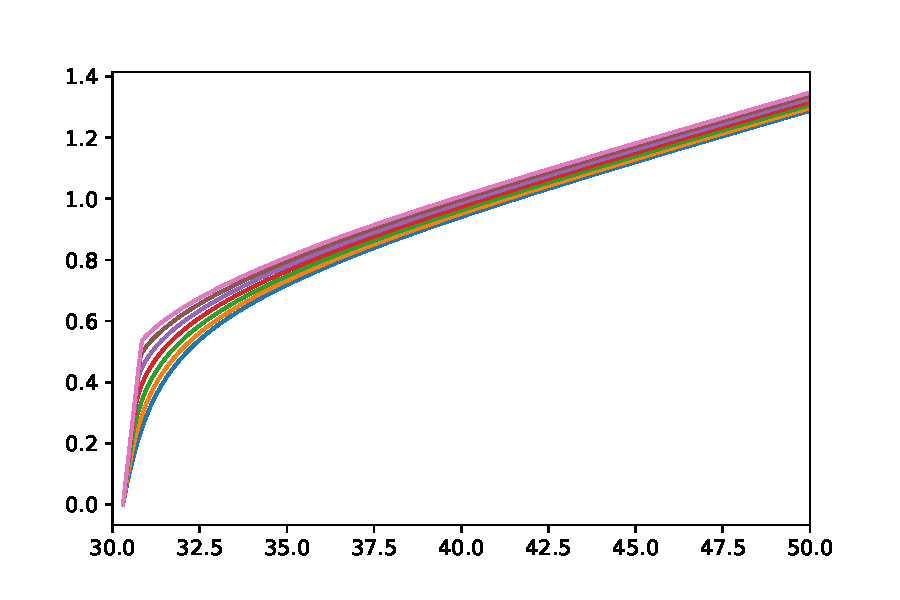
\includegraphics[scale=1]
    {\FigDir/consumption.pdf}
    \caption{The Optimal Consumption Function}
    \label{fig:consumption}
  \end{figure}

  \begin{figure}[H]
      \centering
    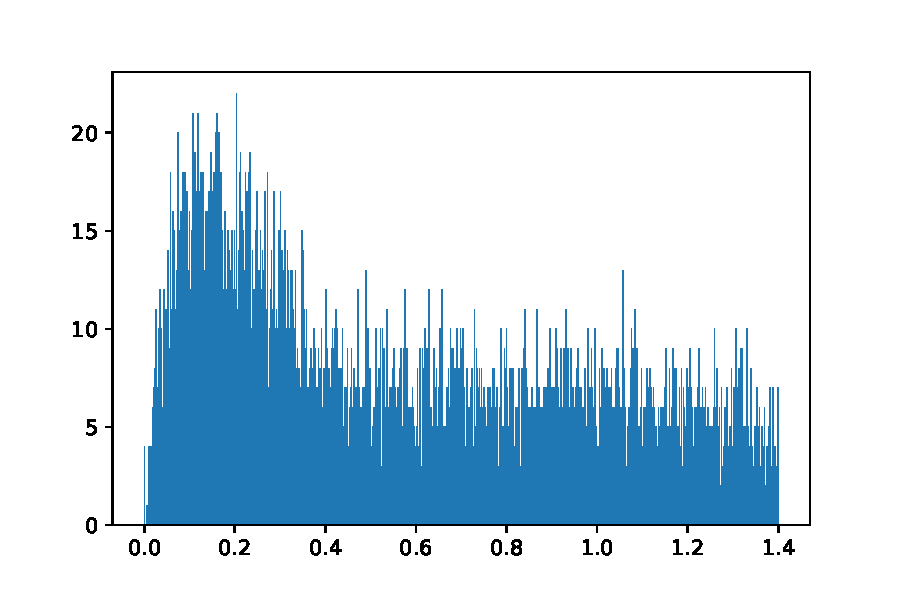
\includegraphics[scale=.9]
    {\FigDir/asset.pdf}
    \caption{The Distribution of Asset}
    \label{fig:asset}
  \end{figure}

  \begin{figure}[H]
      \centering
    \includegraphics[scale=.9]
    {\FigDir/Wealth.pdf}
    \caption{The Distribution of Wealth Level}
    \label{fig:wealth}
  \end{figure}

\clearpage\pagebreak\vfill\eject

\bibliography{LiqConstr,LiqConstr-Add,economics}\end{document}
